\documentclass[12pt]{article}
\usepackage[utf8]{inputenc}
\usepackage{longtable}
\usepackage{multirow}
\usepackage{graphicx}
\graphicspath{ {./author/} }


\renewcommand{\baselinestretch}{1.5}

\title{Alan Mathison Turing(1912-1954)}
\author{Luis Diego Jiménez Delgado}
\date{Agosto 12 del 2019}

\begin{document}

\maketitle

\begin{center}
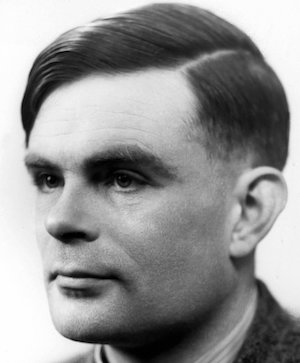
\includegraphics{tu}
\end{center}

Alan Mathison Turing, fue un matemático, lógico, científico de la computación, criptógrafo, filósofo, biólogo teórico, maratoniano y corredor de ultradistancia británico.
Es considerado uno de los padres de la ciencia de la computación y precursor de la informática moderna. Proporcionó una influyente formalización de los conceptos de algoritmo y computación: la máquina de Turing. Formuló su propia versión que hoy es ampliamente aceptada como la tesis de Church-Turing (1936).
Durante la segunda guerra mundial, trabajó en descifrar los códigos nazis, particularmente los de la máquina Enigma, y durante un tiempo fue el director de la sección Naval Enigma de Bletchley Park. Se ha estimado que su trabajo acortó la duración de esa guerra entre dos y cuatro años. Tras la guerra, diseñó uno de los primeros computadores electrónicos programables digitales en el Laboratorio Nacional de Física del Reino Unido y poco tiempo después construyó otra de las primeras máquinas en la Universidad de Mánchester.
En el campo de la inteligencia artificial, es conocido sobre todo por la concepción del test de Turing (1950), un criterio según el cual puede juzgarse la inteligencia de una máquina si sus respuestas en la prueba son indistinguibles de las de un ser humano.
La carrera de Turing terminó súbitamente tras ser procesado por homosexualidad en 1952. Dos años después de su condena, murió —según la versión oficial por suicidio; sin embargo, su muerte ha dado lugar a otras hipótesis, incluida la del asesinato—. El 24 de diciembre de 2013, la reina Isabel II promulgó el edicto por el que se exoneró oficialmente al matemático, quedando anulados todos los cargos en su contra.
\end{document}